\section{Experiments}

\subsection{Ablation Study}
We conducted ablation studies on some of the designs mentioned in Section~\ref{sec:model} to verify their effectiveness.

\begin{figure}[h]
    \centering
    \begin{subfigure}[b]{0.32\textwidth}
        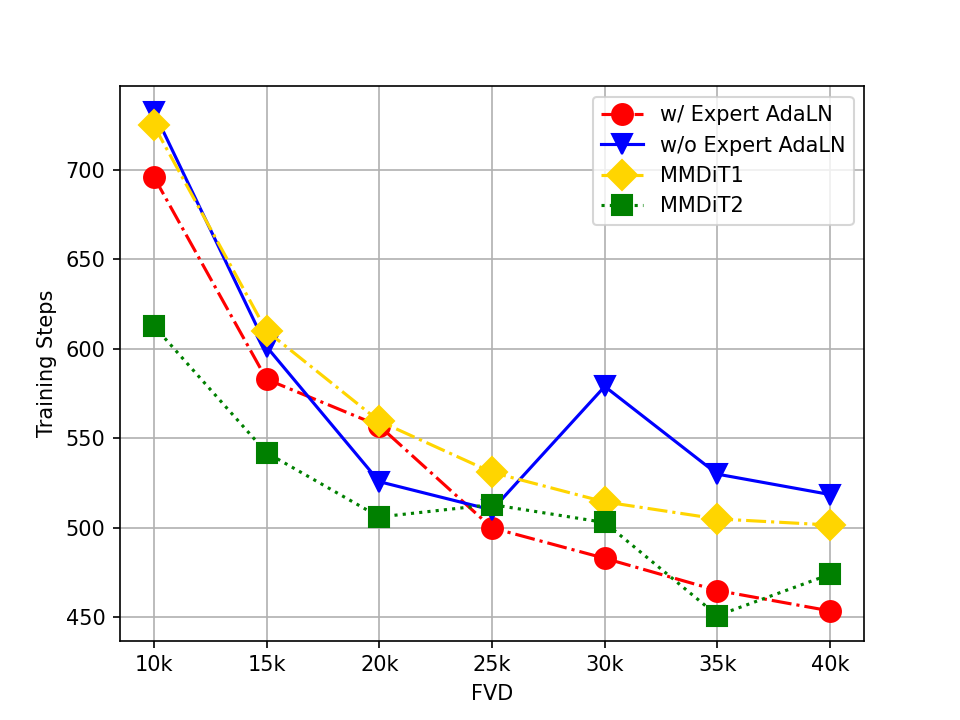
\includegraphics[width=\textwidth]{images/fvd-expert.png}
        \caption{Architecture}
        \label{fig:fvd-expert}
    \end{subfigure}
    \begin{subfigure}[b]{0.32\textwidth}
        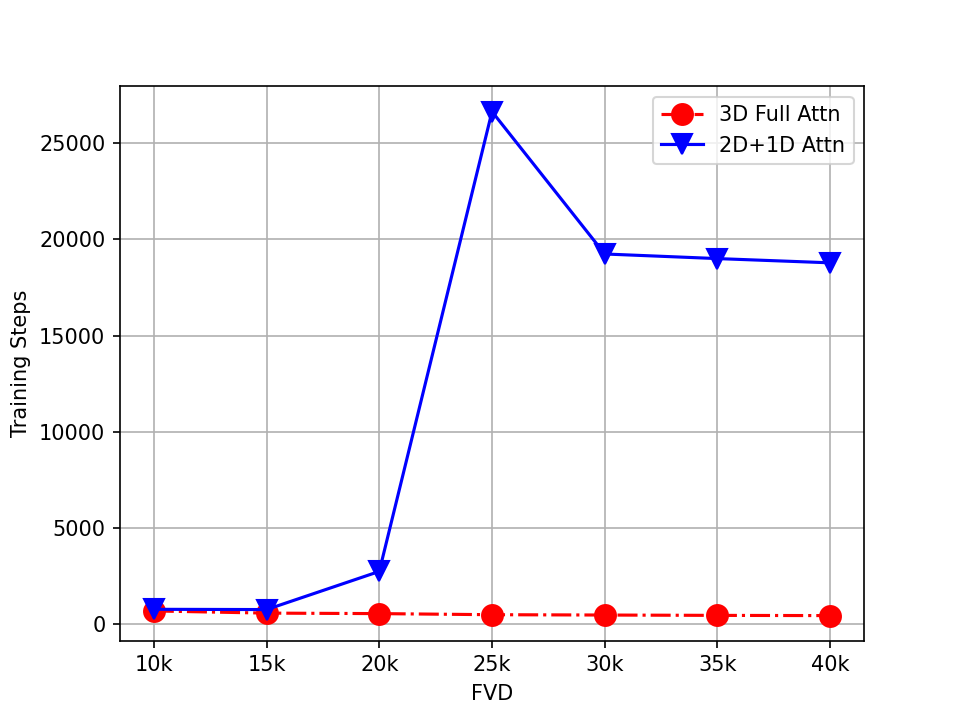
\includegraphics[width=\textwidth]{images/fvd-attn.png}
        \caption{Attention}
        \label{fig:fvd-attn}
    \end{subfigure}
    \begin{subfigure}[b]{0.32\textwidth}
        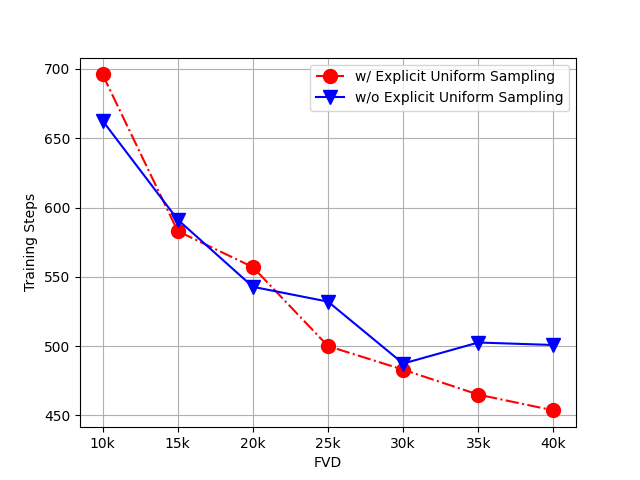
\includegraphics[width=\textwidth]{images/fvd-uniform.png}
        \caption{Explicit Uniform Sampling}
        \label{fig:fvd-uni}
    \end{subfigure}

    \caption{Ablation studies on WebVid test dataset with 500 videos. MMDiT1 has the same number of parameters with the expert AdaLN. MMDiT2 has the same number of layers but twice number of parameters. }
    \label{fig:subfigures}
\end{figure}

\paragraph{Position Embedding.}
We compared 3D RoPE with sinusoidal absolute position embedding. As shown in Figure~\ref{fig:loss-rope-sin} indicates the loss curve of RoPE converges significantly faster than absolute one. This is consistent with the common choice in LLMs.

\paragraph{Expert Adaptive Layernorm.}
We compare three architectures in Figure~\ref{fig:fvd-expert} and Figure~\ref{fig:loss-expert}: MMDiT~\citet{esser2024scaling}, Expert AdaLN, without Expert AdaLN. Cross-attention DiT has been shown to be inferior to MMDiT in~\citep{}, so we don't repeat. According to FVD and loss, expert AdaLN significantly outperforms the model without expert AdaLN and MMDiT with the same number of parameters.
Moreover, the design of Expert AdaLN is more simplified than MMDiT and is closer to current LLMs, making it easier to scale up further.

\paragraph{3D Full Attention.}
In Figure~\ref{fig:fvd-attn} and Figure~\ref{fig:loss-attn} , when we replace 3D full attention with $2D + 1D$ attention, we observe that the model is unstable and prone to collapse.

\paragraph{Explicit Uniform Sampling.}
From Figure~\ref{fig:fvd-uni} and Figure~\ref{fig:loss-uniform-sampling}, we find that using Explicit Uniform Sampling can make a more stable decrease in loss and get a better performance.

\subsection{Evaluation}
% In this section, we present the performance of \model through two primary methods: \textit{automated metric evaluation} and \textit{human assessment}.
% We show results for \model-2B and \model-5B.


%, and will update results for models currently in training.
% The following evaluation defaults to using our largest model to date, 
% The \model-5B model with a high-resolution module can also be accessed via the website \url{https://ChatGLM.cn} or via APIs at \url{https://bigmodel.cn}. 
% To facilitate the development of text-to-video generation, we open-source the model weight at \url{https://github.com/THUDM/CogVideo}.


\subsubsection{Automated Metric Evaluation} 

% \paragraph{Baselines.} 
% We choose openly-accessible top-performing text-to-video models as baselines, including T2V-Turbo~\citep{li2024t2v}, AnimateDiff~\citep{guo2023animatediff}, VideoCrafter2~\citep{chen2024videocrafter2}, OpenSora~\citep{opensora}, Show-1~\citep{zhang2023show}, Gen-2~\citep{gen2}, Pika~\citep{pika}, and LaVie-2~\citep{wang2023lavie}.

\paragraph{VAE Reconstruction Effect}
We compared our 3DVAE with other open-source 3DVAE on $256\times256$ resolution 17-frame videos, using the validation set of the WebVid\citep{Bain21}. On \cref{tab:vae2}, our VAE achieved the best PSNR and exhibited the least jitter. Notably, other VAE methods use fewer latent channels than ours.


\begin{wraptable}{r}{0.5\textwidth}
  \vspace{-3mm}
  \centering
  \caption{Comparison with the performance of other spatiotemporal compression VAEs.}
  \begin{tabular}{cccc}
    \toprule
     & Flickering $\downarrow$ & PSNR $\uparrow$ \\ \midrule
    Open-Sora & 92.4 & 28.5 \\
    Open-Sora-Plan & 90.2 & 27.6 \\
    Ours & \textbf{85.5} & \textbf{29.1} \\ \bottomrule
  \end{tabular}
  \label{tab:vae2}
  \vspace{-3mm}
\end{wraptable}

% \begin{figure}[h]
% \begin{center}
% \includegraphics[width=0.9\linewidth]{images/bench_eval.png}
% \end{center}
% \caption{The radar chart comparing the performance of different models.}
% \label{fig:radar}
% \end{figure}

\hide{
%\begin{wrapfigure}{r}{0.5\textwidth}
\begin{figure}
\centering
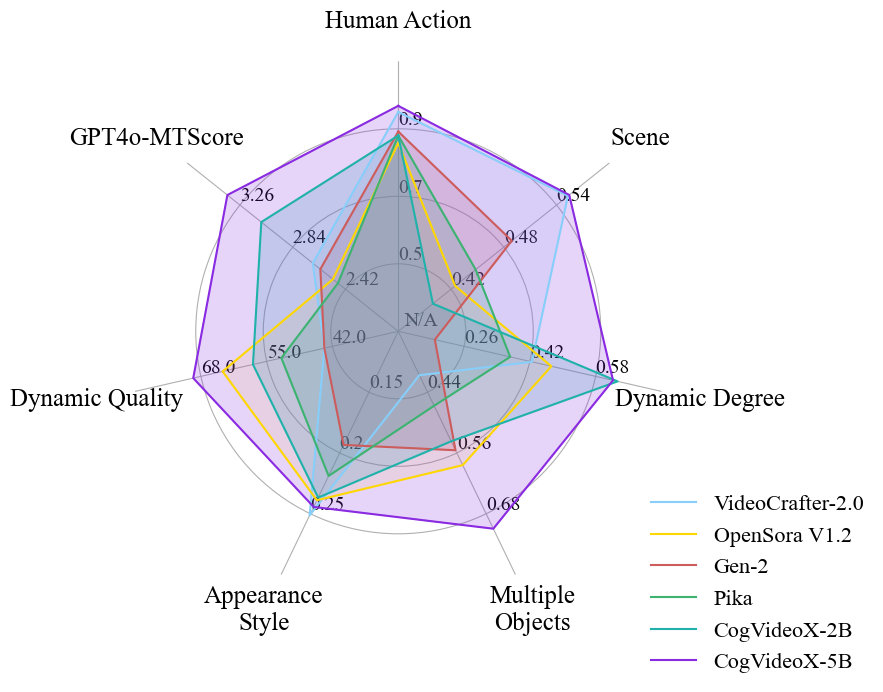
\includegraphics[width=0.7\linewidth]{images/bench_eval9.png}
\caption{The radar chart comparing the performance of different models. CogVideoX represents the largest one. It is clear that CogVideoX outperforms its competitors in the vast majority of metrics, and it is very close to the leading models in the remaining indicator.
}
\label{fig:radar}
% \vspace{-10mm}
%\end{wrapfigure}

\end{figure}

}%end ofhide

\paragraph{Evaluation Metrics.} 
To evaluate the text-to-video generation, we employ several metrics in Vbench~\citep{huang2023vbench} that are consistent with human perception: \emph{Human Action}, \emph{Scene}, \emph{Dynamic Degree}, \emph{Multiple Objects}, and \emph{Appearance Style}. Other metrics, such as color, tend to give higher scores to simple, static videos, so we do not use them.
%VBench is a suite of tools designed to automatically assess the quality of generated videos. We have selected certain metrics from VBench, excluding others that do not align with our evaluation needs. 
%For example, the color metric, intended to measure the presence of objects corresponding to specific colors across frames in the generated video, assesses the model's quality by calculating the probability. 
%However, this metric may mislead video generation models that exhibit greater variation, thus it is not to include it in our evaluation. 

For longer-generated videos, some models might produce videos with minimal changes between frames to get higher scores, but these videos lack rich content. 
Therefore, metrics for evaluating the dynamism become important. 
To address this, we use two video evaluation tools:  \emph{Dynamic Quality}~\citep{liao2024evaluationtexttovideogenerationmodels} and \emph{GPT4o-MTScore}~\citep{yuan2024chronomagic}.

\emph{Dynamic Quality} is defined by the integration of various quality metrics with dynamic scores, mitigating biases arising from negative correlations between video dynamics and video quality.
%leading to a more thorough assessment of video quality. 
GPT4o-MTScore is a metric designed to measure the metamorphic amplitude of time-lapse videos using GPT-4o, such as those depicting physical, biological, and meteorological changes. 
% This metric using GPT-4o~\citep{gpt4o} to score the degree of change, providing a fine-grained assessment of video dynamism. 
%is obtained by extracting frames from the generated videos at regular intervals and using GPT-4o~\citep{gpt4o} to score the degree of change, providing a fine-grained assessment of video dynamism. 
% This method ensures a more accurate evaluation of the content's variability over time, countering the potential bias of static frame sequences in scoring.



\paragraph{Results.} 
Table~\ref{table:results} provides the performance comparison of \model and other models. 
\model-5B achieves the best performance in five out of the seven metrics and shows competitive results in the remaining two metrics. 
These results demonstrate that the model not only excels in video generation quality but also outperforms previous models in handling various complex dynamic scenes. 
In addition, Figure~\ref{fig:radar} presents a radar chart that visually illustrates the performance advantages of \model.



% Please add the following required packages to your document preamble:
% \usepackage[table,xcdraw]{xcolor}
% Beamer presentation requires \usepackage{colortbl} instead of \usepackage[table,xcdraw]{xcolor}
% \usepackage[normalem]{ulem}
% \useunder{\uline}{\ul}{}




% \begin{table}[]

% \centering
% \setlength\tabcolsep{3pt}

% \label{sample-table}
% \small
% \vspace{-10pt}
% \caption{\textbf{Automatic Evaluation Results per Dimension.}The table presents a comparative analysis of various video models across different dimensions. It is evident from the table that, in terms of both human motion and background effects as well as the accuracy and distinctiveness of objects, CogVideoX has achieved the current SOTA level. Furthermore, CogVideoX has garnered a commendable score in the expression of dynamic qualities, a capability that serves as a more precise indicator of the intrinsic properties of video media, distinct from the static nature of photographic images.}

% \vspace{6pt}

% \begin{tabular}{cccccccc}
% \toprule
% \multirow{2}{*}{\textbf{Models} }  & \textbf{human}  & \textbf{object} &\multirow{2}{*}{\textbf{scene}}&\textbf{dynamic} &\textbf{multiple} &\textbf{spatial} &\textbf{appearance} \\
%     & \textbf{action}& \textbf{class}& & \textbf{degree} &\textbf{objects}& \textbf{relationship}&\textbf{style}  
% \\
% \midrule
% CogVideoX & 96.80\% &93.70\% & 55.44\% & 62.22\% & 70.95\% & 61.29\% & 24.44\% \\
% {LaVie-2} & 96.40\% & 97.52\%  & 49.59\% & 31.11\% & 64.88\%  & 38.68\% & 25.09\%  \\
% {T2V-Turbo}  & 95.20\%  & 93.96\%& 55.58\% & 49.17\% & 54.65\%    & 38.67\%  & 24.42\%   \\
% {Gen-2}  & 89.20\%& 90.92\%  & 48.91\%  & 18.89\% & 55.47\%    & 66.91\%   & 19.34\%  \\
% {VideoCrafter-2.0\citep{chen2024videocrafter2}} & 95.00\% & 92.55\% & 55.29\%               & 42.50\% & 40.66\% & 35.86\% & 25.13\%  \\
% {Pika Beta} & 88.00\% & 87.45\%  & 44.80\% & 37.22\% & 46.69\% & 65.65\% & 21.89\%   \\
% AnimateDiff-V2 & 92.60\% & 90.90\%  & 50.19\% & 40.83\%        & 36.88\% & 34.60\%  & 22.42\%\\
% {OpenSora V1.2}   & 85.80\% & 83.37\%& 42.47\%   & 47.22\%    & 58.41\% & 67.51\%  & 23.89\%  \\
% {Show-1} & 95.60\%  & 93.07\%  & 47.03\% & 44.44\% & 45.47\% & 53.50\%  & 23.06\%  \\
% {HiGen}  & 86.20\%  & 86.06\%  & 44.88\% & 99.17\% & 22.39\%  & 22.43\% & 24.54\% \\  
% \bottomrule
% \end{tabular}
% \end{table}



% \iffalse



% \begin{table}[ht!]
% \centering
% \caption{Evaluation results.}
% \setlength\tabcolsep{3pt}
% \label{sample-table}
% \begin{center}
% \small
% \resizebox{0.9\linewidth}{!}{
% \begin{tabular}{ccccccccc}

% \multirow{2}{*}{\textbf{Models} }  & \textbf{subject}  & \textbf{background} &\textbf{temporal} &\textbf{motion} &\textbf{dynamic} &\textbf{aesthetic} &\textbf{imaging} &\textbf{object} \\
%     & \textbf{consistency}& \textbf{consistency}& \textbf{flickering}& \textbf{smoothness} &\textbf{degree}& \textbf{quality}&\textbf{quality} & \textbf{class}
% \\ \hline 
%         CogVideoX & 94.66\% & 95.92\% & 97.47\% & 98.10\% & 62.22\% & 55.14\% & 63.62\% & 93.70\%  \\
%         LaVie-2 & 97.90\% & 98.45\% & 98.76\% & 98.42\% & 31.11\% & 67.62\% & 70.39\% & 97.52\%  \\ 
%         T2V-Turbo (VC2) & 96.28\% & 97.02\% & 97.48\% & 97.34\% & 49.17\% & 63.04\% & 72.49\% & 93.96\%  \\ 
%         Gen-2 (2023-06) & 97.61\% & 97.61\% & 99.56\% & 99.58\% & 18.89\% & 66.96\% & 67.42\% & 90.92\%  \\ 
%         VideoCrafter-2.0\citep{chen2024videocrafter2} & 96.85\% & 98.22\% & 98.41\% & 97.73\% & 42.50\% & 63.13\% & 67.22\% & 92.55\%  \\ 
%         Pika Beta (2023-06) & 96.76\% & 98.95\% & 99.77\% & 99.51\% & 37.22\% & 63.15\% & 62.33\% & 87.45\%  \\ 
%         AnimateDiff-V2 & 95.30\% & 97.68\% & 98.75\% & 97.76\% & 40.83\% & 67.16\% & 70.10\% & 90.90\%  \\ 
%         OpenSora V1.2 & 94.45\% & 97.90\% & 99.47\% & 98.20\% & 47.22\% & 56.18\% & 60.94\% & 83.37\%  \\ 
%         Show-1 & 95.53\% & 98.02\% & 99.12\% & 98.24\% & 44.44\% & 57.35\% & 58.66\% & 93.07\%  \\ 
%         HiGen & 90.07\% & 93.99\% & 93.24\% & 96.69\% & 99.17\% & 57.30\% & 63.92\% & 86.06\% \\ 
% \hline \\

% \multirow{2}{*}{\textbf{Models} }  & \textbf{multiple}  & \textbf{human} &\multirow{2}{*}{\textbf{color}} &\textbf{spatial} &\multirow{2}{*}{\textbf{scene}} &\textbf{appearance} &\textbf{temporal} &\textbf{overall} \\
%     & \textbf{objects}& \textbf{action}& & \textbf{relation} & & \textbf{style}&\textbf{style} & \textbf{consistency}
% \\ \hline 
%         CogVideoX & 70.95\% & 96.80\% & 79.75\% & 61.29\% & 55.44\% & 24.44\% & 23.69\% & 26.73\%  \\ 
%         LaVie-2 & 64.88\% & 96.40\% & 91.65\% & 38.68\% & 49.59\% & 25.09\% & 25.24\% & 27.39\%  \\ 
%         T2V-Turbo (VC2) & 54.65\% & 95.20\% & 89.90\% & 38.67\% & 55.58\% & 24.42\% & 25.51\% & 28.16\%  \\
%         Gen-2 (2023-06) & 55.47\% & 89.20\% & 89.49\% & 66.91\% & 48.91\% & 19.34\% & 24.12\% & 26.17\%  \\ 
%         VideoCrafter-2.0 & 40.66\% & 95.00\% & 92.92\% & 35.86\% & 55.29\% & 25.13\% & 25.84\% & 28.23\%  \\
%         Pika Beta (2023-06) & 46.69\% & 88.00\% & 85.31\% & 65.65\% & 44.80\% & 21.89\% & 24.44\% & 25.47\%  \\ 
%         AnimateDiff-V2 & 36.88\% & 92.60\% & 87.47\% & 34.60\% & 50.19\% & 22.42\% & 26.03\% & 27.04\%  \\ 
%         OpenSora V1.2 & 58.41\% & 85.80\% & 87.49\% & 67.51\% & 42.47\% & 23.89\% & 24.55\% & 27.07\%  \\ 
%         Show-1 & 45.47\% & 95.60\% & 86.35\% & 53.50\% & 47.03\% & 23.06\% & 25.28\% & 27.46\%  \\ 
%         HiGen & 22.39\% & 86.20\% & 86.22\% & 22.43\% & 44.88\% & 24.54\% & 25.14\% & 27.14\% \\ \hline

% \hline \\
% \end{tabular}

% }
% \end{center}
% \end{table}

% \fi






% \begin{table}[!ht]
% \centering

% \label{sample-table}
% \small
% \vspace{-10pt}
% \caption{\textbf{Automatic Evaluation Results per Dimension.}}

% \vspace{6pt}

% \resizebox{0.8\linewidth}{!}{
%     \begin{tabular}{cccc}
%         \textbf{Models} & \textbf{\Centerstack{Dynamics Range}} & \textbf{\Centerstack{Dynamics Controllability}} & \textbf{\Centerstack{Dynamics-based Quality}} \\ \hline
%         CogVideoX       & 55.7 & 71.8 & \textbf{69.5} \\ 
%         Gen-2           & 30.8 & \textbf{82.5} & 43.6 \\ 
%         Pika            & 43.2 & 72.0 & 52.1 \\ 
%         VideoCrafter2   & 34.1 & 57.0 & 43.6 \\ 
%         OpenSora        & \textbf{61.2} & 62.4 & 63.7 \\ 
%         Show-1          & 45.1 & 73.9 & 57.7 \\ 
%     \end{tabular}
% }
% \end{table}


% \begin{figure}[h]
% \begin{center}
% \includegraphics[width=0.9\linewidth]{images/bench_eval.png}
% \end{center}
% \caption{The radar chart comparing the performance of different models.}
% \label{fig:radar}
% \end{figure}

\hide{
%\begin{wrapfigure}{r}{0.5\textwidth}
\begin{figure}
\centering
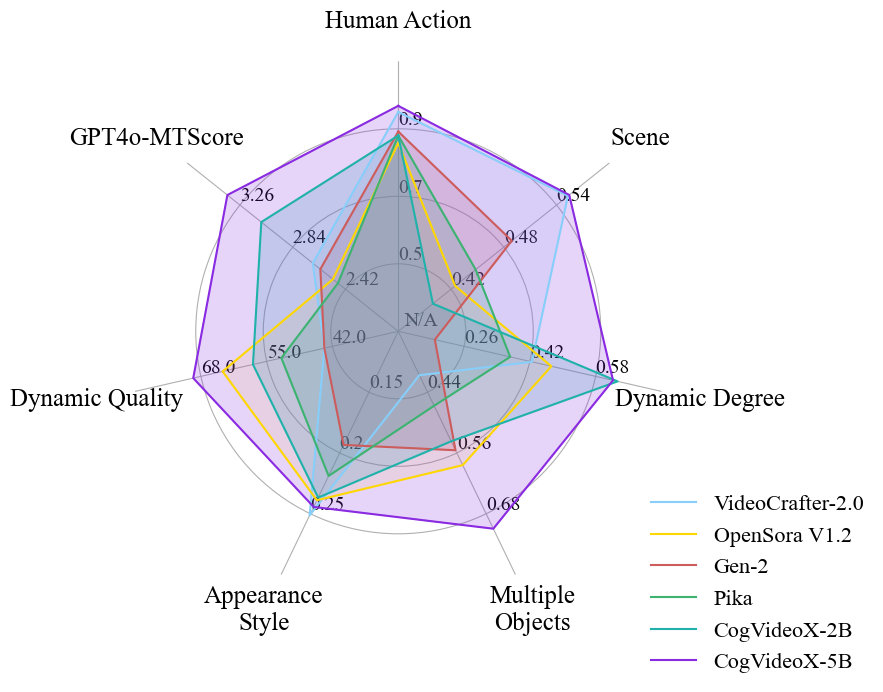
\includegraphics[width=0.7\linewidth]{images/bench_eval9.png}
\caption{The radar chart comparing the performance of different models. CogVideoX represents the largest one. It is clear that CogVideoX outperforms its competitors in the vast majority of metrics, and it is very close to the leading models in the remaining indicator.
}
\label{fig:radar}
% \vspace{-10mm}
%\end{wrapfigure}

\end{figure}

}%end ofhide


\subsubsection{Human Evaluation}

In addition to automated scoring mechanisms, we also establish a comprehensive human evaluation framework to assess the general capabilities of video generation models. Evaluators will score the generated videos on four aspects: Sensory Quality, Instruction Following, Physics Simulation, and Cover Quality, using three levels: 0, 0.5, or 1. Each level is defined by detailed guidelines. The specific details are provided in the Appendix~\ref{sec:human_evalution}.

We compare Kling (2024.7), one of the best closed-source models, with \model-5B under this framework. The results shown in Table~\ref{table:human_eva} indicate that \model-5B wins the human preference over Kling across all aspects. 

\begin{table}[!ht]
\centering
\label{sample-table}
\small
\vspace{-5pt}
\caption{Human evaluation between CogVideoX and Kling.}
\label{table:human_eva}
\resizebox{0.75\linewidth}{!}{
    \begin{tabular}{cccccc}
    \toprule
        Model & \Centerstack{Sensory\\Quality} & \Centerstack{Instruction\\Following}&\Centerstack{Physics\\Simulation} & \Centerstack{Cover\\Quality} & 
        \Centerstack{Total\\Score} \\ 
        \midrule
        Kling & 0.638 & 0.367 & 0.561 & 0.668 & 2.17 \\
        \midrule
         {\bf CogVideoX-5B} & {\bf 0.722} & {\bf 0.495} & {\bf 0.667} & {\bf 0.712} & {\bf 2.74}  \\
        \bottomrule
    \end{tabular}
}
\vspace{-3mm}
\end{table}



% \begin{table}[!ht]
% \centering

% \label{sample-table}
% \small
% \vspace{-10pt}
% \caption{\textbf{Automatic Evaluation Results per Dimension.}}

% \vspace{6pt}

% \resizebox{0.8\linewidth}{!}{
%     \begin{tabular}{cccc}
%         \textbf{Models} & \textbf{\Centerstack{Dynamics Range}} & \textbf{\Centerstack{Dynamics Controllability}} & \textbf{\Centerstack{Dynamics-based Quality}} \\ \hline
%         CogVideoX       & 55.7 & 71.8 & \textbf{69.5} \\ 
%         Gen-2           & 30.8 & \textbf{82.5} & 43.6 \\ 
%         Pika            & 43.2 & 72.0 & 52.1 \\ 
%         VideoCrafter2   & 34.1 & 57.0 & 43.6 \\ 
%         OpenSora        & \textbf{61.2} & 62.4 & 63.7 \\ 
%         Show-1          & 45.1 & 73.9 & 57.7 \\ 
%     \end{tabular}
% }
% \end{table}
